\documentclass[a4paper,11pt]{jsarticle}


% 数式
\usepackage{amsmath,amsfonts}
\usepackage{bm}
% 画像
\usepackage[dvipdfmx]{graphicx}

% urlなど
\usepackage{url}
\usepackage{float}

\begin{document}

\title{ダイクストラ法を用いた、ポリゴン上の最短経路検索}
\author{Ito Takeru}
\date{\today}
\maketitle




\section{概要}
今回の実験は、PLYファイルとして与えられたポリゴンデータから、頂点とエッジの情報を取り出し、ダイクストラ法にかけることでポリゴンの表面上で疑似的な最短経路計算を行うというものである。

\section{原理}

以下に今回の実験で用いられる用語について解説する。

ダイクストラ法とは、重みのついたグラフ上の最短経路問題を解くためのアルゴリズムである(例: 図\ref{dijikstra}参照)。

\begin{figure}[H]
  \centering
  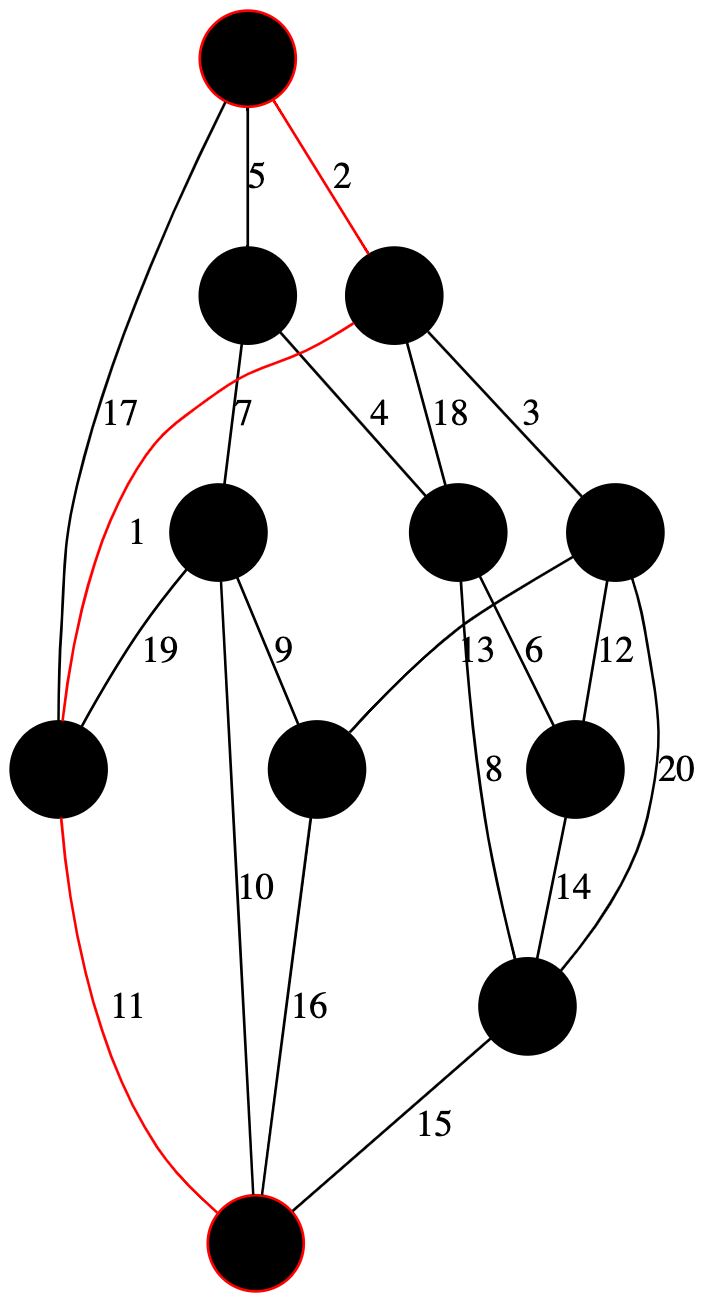
\includegraphics[scale = 0.15]{../Figs/dijkstra.png} 
  \caption{ダイクストラ法を適用した例}
  \label{dijikstra}
\end{figure}

次にPLYファイルについて述べる

PLY (Python Lex-Yacc) は、3Dモデリングソフトウェアなどで使用されるファイルフォーマットである\cite{ply}。
PLYファイルは、頂点と面の情報の情報が入力されており、CADやmeshlabなどの3Dオブジェクトを扱うツールで読み込むことができる。

\section{実験手順}

\subsection{最短経路の描画}

まず、PLYファイルとしてwebサイト上で公開されていたplyファイル、helix.plyを利用した(図\ref{helix})

\begin{figure}[H]
  \centering
  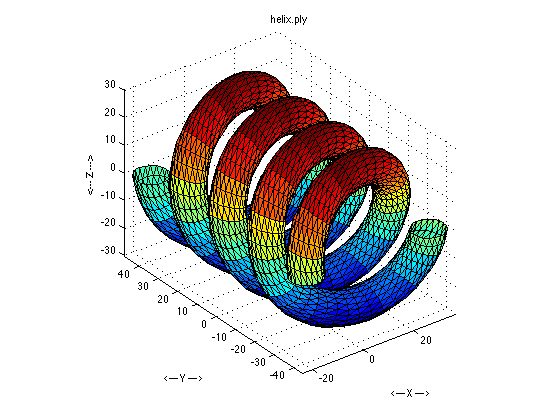
\includegraphics[scale = 0.5]{../Figs/helix.png} 
  \caption{helix}
  \label{helix}
\end{figure}

次にPythonを用いてこのファイルからノードとして頂点情報を、エッジとしてポリゴンの三角形の辺の情報を抜き出し、エッジの重みとして辺の長さを使うことでグラフの情報を取り出した。
そして、できたグラフデータのノードの内2つを、スタートとゴールのノードに指定し、C言語のダイクストラ法のアルゴリズムをを実行し、重みの最も少ないノードの順序を求めた。

\subsection{隣接行列と優先度キューによるダイクストラ法の実行速度比較}

同様に\cite{fsu}において公開されている3つのPLYデータairplane, teapot, apple(図\ref{apple, teapot, airplane})において、全ての点の組間で、隣接行列に基づいたダイクストラ法と優先度キューに基づいたダイクストラ法を実施したときの計算量を比較した。
また、それぞれの図形のノード、エッジ数は表\ref{node-edge}の通りであり、計算量はプログラムの繰り返し処理ごとに+1されるような変数を用意してカウントした。

\begin{figure}[H]
  \centering
  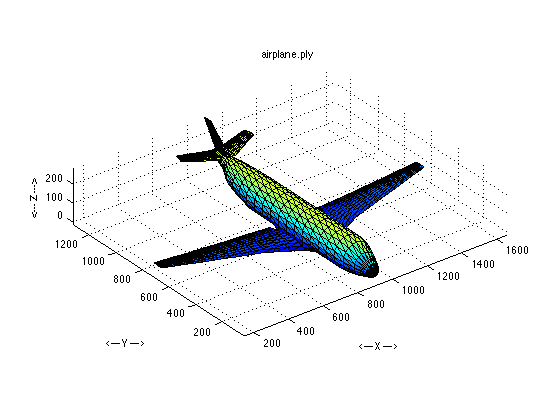
\includegraphics[scale = 0.8]{../Figs/airplane.png} 
  \caption{airplaneの図}
  \label{airplane}
\end{figure}

\begin{figure}[H]
  \centering
  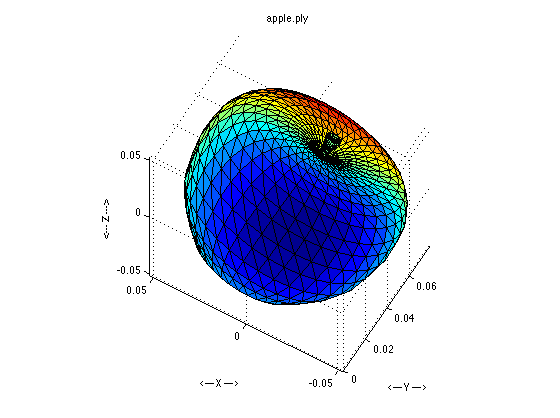
\includegraphics[scale = 0.8]{../Figs/apple.png} 
  \caption{appleの図}
  \label{apple}
\end{figure}

\begin{figure}[H]
  \centering
  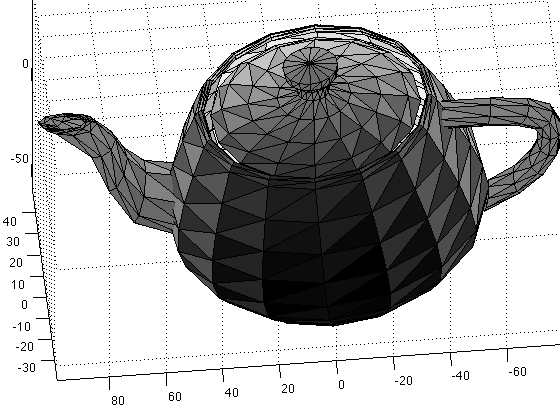
\includegraphics[scale = 0.8]{../Figs/teapot.png} 
  \caption{teapotの図}
  \label{teapot}
\end{figure}


\begin{table}[H]
  \centering\begin{tabular}{ccc}
  図形 & ノード数 & エッジ数 \\
  \hline
  airplane & 1335 & 3789 \\
  apple & 867 & 2568 \\
  teapot & 1177 & 3432 \\
  \hline
  \end{tabular}
  \caption{3つの図形のノード、エッジのステータス}
  \label{node-edge}
\end{table}


\section{結果}

\subsection{最短経路の描画}

ダイクストラ法を実装した結果を、Pythonを用いて可視化すると以下のようなことが分かった。
図\ref{helix-path1}, \ref{helix-path2}を見ると点は螺旋の内側を通っており、正しく最短に近い経路を取っていることが分かった。
しかし、図\ref{helix-path2}に良く表れているように、検出した経路に折れ曲がりが見られ、ポリゴン表面上における本当の最短経路ではないことがわかる。

\begin{figure}[H]
  \centering
  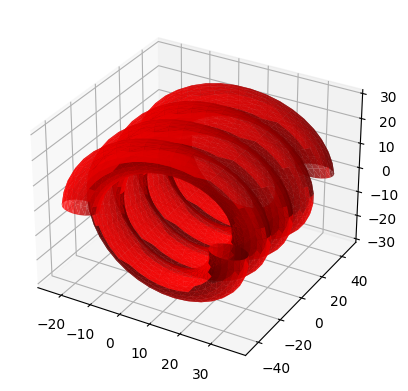
\includegraphics[scale = 1.0]{../Figs/red-helix.png}
  \caption{元のhelix}
  \label{red-helix}
\end{figure}

\begin{figure}[H]
  \centering
  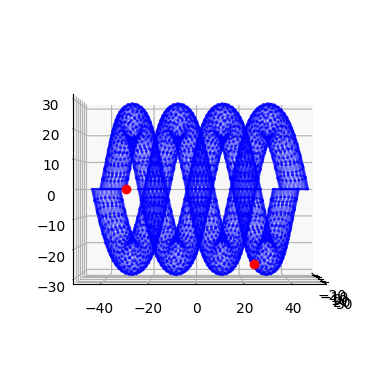
\includegraphics[scale = 1.0]{../Figs/helix-0to634-endpoints.png}
  \caption{ノードとエッジに分解されたポリゴンと設定した始点と終点}
  \label{helix-endpoints}
\end{figure}

\begin{figure}[H]
  \centering
  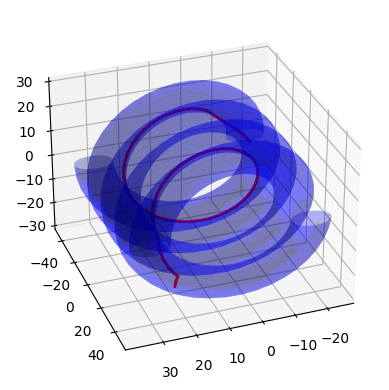
\includegraphics[scale = 1.0]{../Figs/helix-0to634-1.png} 
  \caption{ダイクストラ法によって求めた最短経路}
  \label{helix-path1}
\end{figure}

\begin{figure}[H]
  \centering
  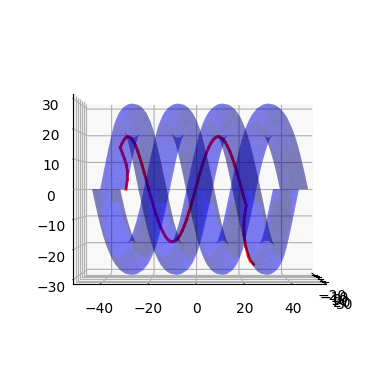
\includegraphics[scale = 1.0]{../Figs/helix-0to634-2.png} 
  \caption{ダイクストラ法によって求めた最短経路}
  \label{helix-path2}
\end{figure}

\subsection{隣接行列と優先度キューを用いたダイクストラ法の比較}

隣接行列を用いたダイクストラ法と、優先度キューを用いたダイクストラ法をグラフの全ての点間で実施したときの、1組の点間におけるダイクストラ法の平均計算量は以下のようになった。

\begin{table}[H]
  \centering\begin{tabular}{ccccc}
  図形 & ノード数 & エッジ数 & dijkstra(優先度キュー) & dijkstra(隣接行列) \\
  \hline
  apple & 867 & 2568 & 35523 & 641016 \\
  airplane & 1335 & 3789 & 23101 & 434551 \\
  teapot & 1177 & 3432 & 30956 & 648059 \\
  \hline
  \end{tabular}
  \caption{図形とグラフ構造ごとの計算量比較}
  \label{graph-calc}
\end{table}

\section{考察}

最短経路の可視化を通してわかったことを述べる。
まず、この最短経路は通れる場所が頂点とエッジのみであることから、表面全体における最短経路とは異なった所を通ることが予想できるが、
今回の例で行った範囲で考えると、かなり表面全体における最短経路に近い経路を通ることが分かった。
また、今後の展望としては以下のようなものが考えられた。

\begin{itemize}
  \item ポリゴンをどのように細分化していったら、ダイクストラ法の結果は真の最短経路に収束するのか
  \item 曲面上に幾何学的なパターンのポリゴンを構成することで幾何の接続のような概念を疑似的に表せないか
\end{itemize}

隣接行列と優先度キューのダイクストラ法アルゴリズムを比較して考えたことをのべる。
表を見ると、appleはノード、エッジ数が他の図形に比べて少ないにもかかわらずairplaneよりも多く、teapotと同程度の計算量を要した。
これは、図形の連結性に原因があり、teapotは蓋と容器、airplaneは翼と胴体は繋がっておらず、そのためこれらのダイクストラ法のアルゴリズムは途中で打ち切られたことが原因だと考えられる。
特に、連結していないことの判定において、ある点に対して暫定距離が最小のノードを取り出す際に、優先度キューならばrootのノードの暫定距離が INTMAX であること、隣接行列なら、visitedノードがtrueなノードの全てを確認しその中のノードが全ての距離が確定済であること、を条件にする。
このことから、優先度キューのほうが連結でないことをより少ない計算量で判定することができると考えられる。
これがappleにおける優先度キューのダイクストラ法計算量が、他の図形の優先度キューに比べて大きいという結果に表れたと考えられる。

全ての図形において、優先度キューのほうが隣接行列よりも計算量が小さかった。
これは、ポリゴンが成立する条件により、グラフが常に疎行列であるからだと考えられる。
また、1つのノードに繋がっているエッジの数をnとすると、それぞれの計算量に以下の関係が成り立ち、このことも結果を裏づけていると言える。
まず以下が成立。

\begin{align}
V \approx \frac{2E}{n}
\end{align}

よって、隣接リストの計算量は

\begin{align}
  O((V+E)\log V) \approx O(V \log V)
\end{align}

そして、隣接行列の計算量は

\begin{align}
  O(V^2+E) \approx O(V^2)
\end{align}

このことからポリゴン上のダイクストラ法において、一般的に隣接リストの方が計算量が少ないことが分かる。


\begin{thebibliography}{9}
  \bibitem {ply} Paul Bourke. PLY - Polygon File Format. \url{http://paulbourke.net/dataformats/ply/}
  \bibitem {fsu} FSU. PLY Files an ASCII Polygon Format \url{https://people.sc.fsu.edu/~jburkardt/data/ply/ply.html}
\end{thebibliography}



\end{document}